\documentclass[12pt,a4paper]{article}

\usepackage[utf8]{inputenc}
\usepackage[brazilian]{babel}
\usepackage{amsmath}
\usepackage{graphicx}
\usepackage{longtable}
\usepackage{siunitx}
\usepackage{booktabs}
\usepackage{geometry}
\usepackage{float}
\usepackage{indentfirst}
\usepackage{newtxtext}
\usepackage{newtxmath}

\usepackage[authoryear]{natbib}

\geometry{margin=2.5cm}

\title{Análise do Movimento Harmônico Amortecido}
\author{Enzo Rocha Leite Diniz Ribas \\ Centro Federal de Educação Tecnológica de Minas Gerais}
\date{\today}

\begin{document}
\begin{titlepage}

\begin{center}


\includegraphics[width=4cm]{media/Logo_CEFET-MG.png}

\Large
Centro Federal de Educação Tecnológica de Minas Gerais

\vspace{1cm}

\Large
Curso de Engenharia Mecânica

\vspace{2cm}

\Huge
Análise do Movimento Harmônico Amortecido

\vspace{3cm}

\begin{flushright}
\Large
Mecânica, Oscilações, Fluidos e Termodinâmica, Turma T03 \\
Prof. Dr. Mauro Lucio Lobão Iannini
\end{flushright}

\vspace{3cm}

\large
Enzo Rocha Leite Diniz Ribas (Eng. Mecânica - 20253002819)\\
Gabriel Resende Amorim Oliveira (Eng. Elétrica - 20233014438)\\
Leandro Césari e Silva Barros (Eng. Mecânica - 20253005104)\\

\vfill

\Large
Belo Horizonte

\Large
\the\year/{1}

\end{center}

\end{titlepage}

\section{Introdução}

O roteiro do experimento \citep{Roteiro_Experimento_05} propõe a análise do movimento harmônico amortecido com o objetivo de ``Analisar a dependência com o tempo da amplitude do movimento harmônico de um sistema massa-mola amortecido'' e ``determinar o coeficiente de amortecimento e outras constantes descritivas do movimento oscilatório''.

\section{Fundamentação Teórica}

Considere um sistema constituído por um corpo de prova de massa total $m$ acoplado a uma mola helicoidal de constante elástica $k$, suspenso verticalmente sob a ação de um campo gravitacional uniforme.

\begin{figure}[H]
\centering
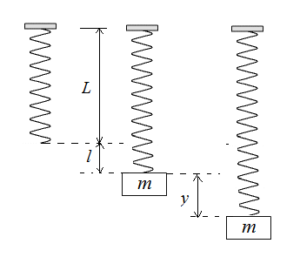
\includegraphics[width=0.8\textwidth]{media/graphs/spring_fbd}
\caption{Diagrama de um sistema de pêndulo simples. Fonte: \cite{the_vibration_of_vertical_spring_2020}}
\label{fig:free_body_diagram}
\end{figure}

Quando o conjunto é transladado de sua posição de equilíbrio estável por uma coordenada espacial $y$, atua sobre ele uma força restauradora conservativa regida pela Lei de Hooke, a força elastíca, expressa por:

\begin{equation}
    F_{\text{el}} = -k y
\end{equation}

Denotamos $y(t)$ como a posição do corpo de prova em função do tempo, onde $y=0$ corresponde à posição de equilíbrio. A força restauradora é proporcional ao deslocamento $y$ e atua na direção oposta, buscando retornar o sistema à posição de equilíbrio.

A força gravitacional $w = mg$ atua sobre o corpo de prova. Então $y(t)$ está relacionado com forças que agem sobre a massa pela lei de Newton,

\begin{equation}
    m\frac{d^2y(t)}{dt^2} = f(t),
\end{equation}

em que $f(t)$ é a força total sobre o corpo de prova e $\frac{d^2y(t)}{dt^2}$ é a aceleração do corpo de prova, que é a segunda derivada temporal da posição.

Na dinâmica do sistema, além da força peso e da força elástica, é importante considerar a presença de forças externas, como forças de atrito ou resistência do ar, que atuam como forças dissipativas, causando a perda de energia do sistema ao longo do tempo.

A força de amortecimento, $F_{\text{am}}$ causada pela resistência do ar, é uma força dissipativa que atua na direção oposta ao movimento do corpo de prova, reduzindo a amplitude das oscilações ao longo do tempo. Essa força de resistência é proporcial à velocidade escalar $\frac{d y}{d t}$ da massa; em geral é chamado de \textbf{amortecimento viscoso} \citep{boycediprima2024}.

\begin{equation}
    F_{\text{am}} = -\gamma \frac{d y(t)}{d t}
\end{equation}

em que $\gamma$ é o coeficiente de amortecimento, que depende das propriedades do fluido e da geometria do corpo de prova.

Pode ser aplicada uma força externa $F_{\text{ext}}(t)$ ao sistema, que pode ser uma força periódica ou um impulso. Levando essas quatro forças em consideração, a força total $f(t)$ que atua sobre o corpo de prova é dada por:

\begin{align*}
    f(t) &= m\frac{d^2y(t)}{dt^2} \\
    m\frac{d^2y(t)}{dt^2} &= w + F_{\text{el}} + F_{\text{am}} + F_{\text{ext}}(t) \\
    &= mg - ky - \gamma\frac{dy}{dt} + F_{\text{ext}}(t)
\end{align*}

Pela segunda lei de Newton, a força peso $w$ é equilibrada pela força elástica $F_{\text{el}}$ na posição de equilíbrio, ou seja, $mg = ky_{eq}$, em que $y_{eq}$ é a posição de equilíbrio. Assim, podemos redefinir a coordenada $y$ para que $y=0$ corresponda à posição de equilíbrio, eliminando o termo constante $mg$ da equação.

\begin{align*}
    m\frac{d^2y(t)}{dt^2} &= -ky - \gamma\frac{dy}{dt} + F_{\text{ext}}(t) \\
    m\frac{d^2y(t)}{dt^2} + \gamma\frac{dy}{dt} + ky &= F_{\text{ext}}(t)
\end{align*}

Podemos reescrever a equação utilizando a frequência angular natural da vibração do sistema massa-mola, definida por $\omega_0 = \sqrt{\frac{k}{m}}$, e o coeficiente de amortecimento por unidade de massa, definido por $\beta = \frac{\gamma}{2m}$, e considerando a força externa nula, $F_{\text{ext}}(t) = 0$, para obter a equação do movimento harmônico amortecido:

\begin{align*}
    m\frac{d^2y(t)}{dt^2} + \gamma\frac{dy}{dt} + ky &= 0\\
    \frac{d^2y}{dt^2} + \frac{\gamma}{m}\frac{dy}{dt} + \frac{k}{m}y &= 0 \\
    \frac{d^2y}{dt^2} + 2\beta\frac{dy}{dt} + \omega_0^2 y &= 0
\end{align*}
que é uma Equação Diferencial Ordinária Linear de Segunda Ordem, homogênea, com coeficientes constantes.

Podemos interpretar os termos da EDO da seguinte maneira, o termo $\frac{d^2y}{dt^2}$ representa a tendência do sistema a manter seu estado de movimento, o termo $2\beta\frac{dy}{dt}$ representa a força de amortecimento que atua para reduzir a velocidade do sistema, e o termo $\omega_0^2 y$ representa a força restauradora que atua para retornar o sistema à posição de equilíbrio.

No escopo deste experimento, configura-se o regime de **Subamortecimento**, caracterizado pela restrição dinâmica $\gamma < \omega_0$. Sob esta condição, a solução geral da EDO é dada por:

\begin{equation}
    y(t) = A e^{-\beta t} \cos(\omega t + \phi)
\end{equation}

Que será a função utilizada como base para o ajuste dos dados experimentais.

\section{Metodologia}

O experimento foi realizado utilizando um sistema massa-mola amortecido, composto por uma mola helicoidal, um corpo de prova de massa total $m$, e um sensor de movimento para registrar a posição do corpo de prova ao longo do tempo. O sistema foi configurado para oscilar verticalmente, e a aquisição de dados foi realizada utilizando o software \textit{DataStudio}.

\begin{figure}[H]
\centering
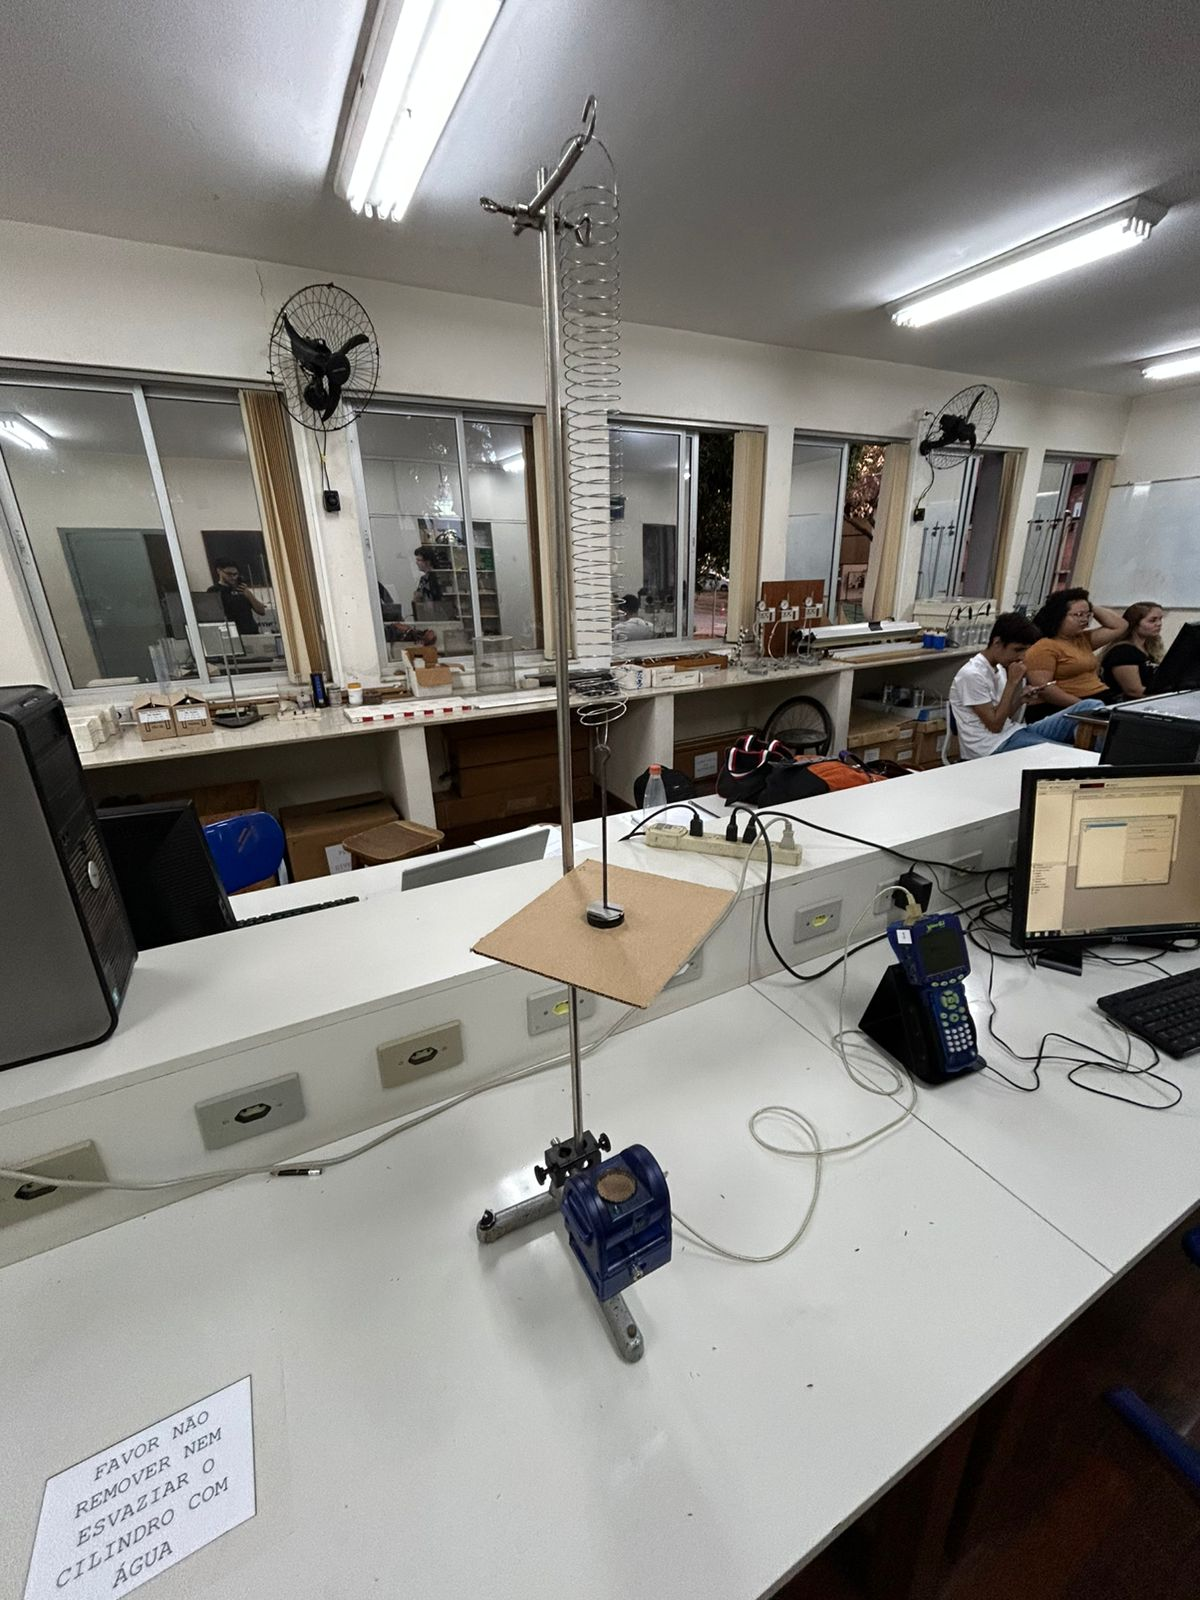
\includegraphics[width=0.8\textwidth]{media/photos/sistema}
\caption{Sistema de massa-mola amortecido. Fonte: Autor}
\label{fig:pendulo_experimento}
\end{figure}

\begin{figure}[H]
\centering
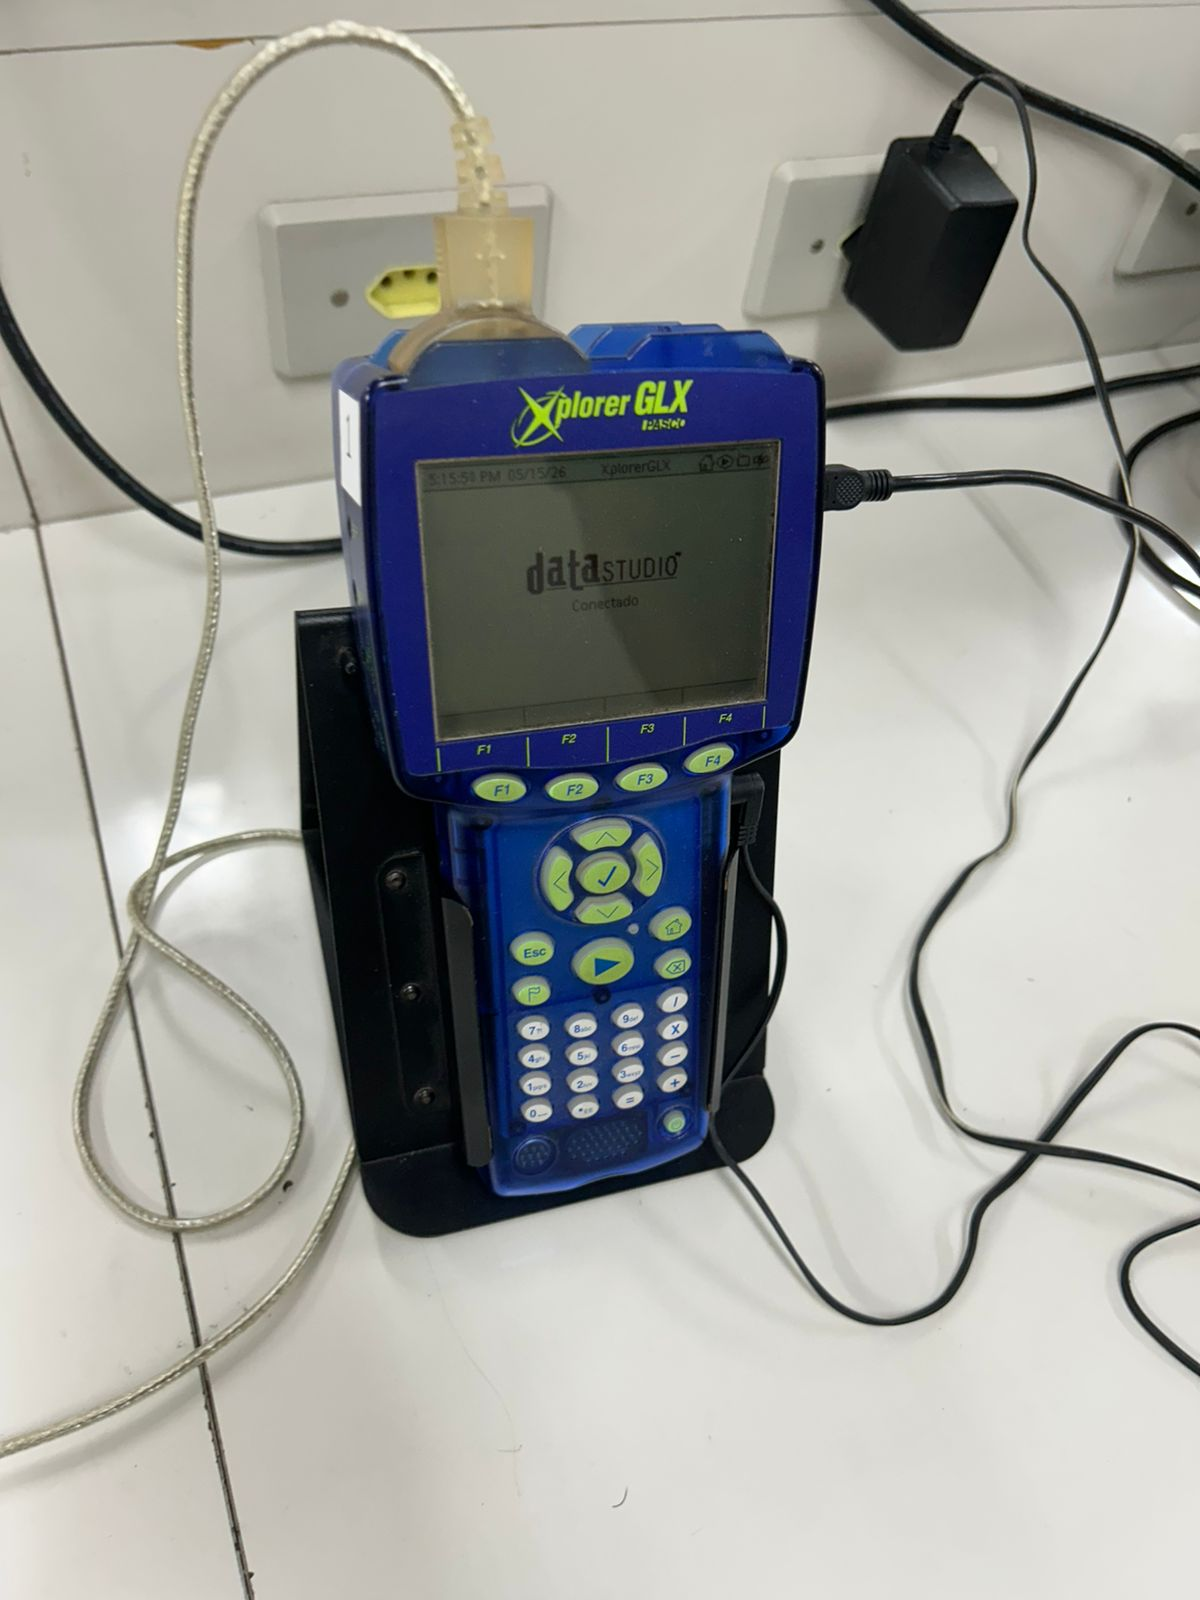
\includegraphics[width=0.8\textwidth]{media/photos/datastudio}
\caption{DataStudio. Fonte: Autor}
\label{fig:datastudio}
\end{figure}

\section{Procedimentos}

O procedimento experimental seguiu as seguintes etapas:

\subsection{Construção do experimento}

O sistema foi configurado de maneira que o sistema massa-mola esteja bem fixado e o sensor esteja posicionado de modo a garantir a leitura de todo o movimento, sem obstruções ou interferências.

A frequência utilizada para a aquisição de dados foi de \(100\,\text{Hz}\), o que é suficiente para capturar o movimento oscilatório do sistema massa-mola com precisão.

\subsection{Aquisição do movimento}

O movimento oscilatório foi iniciado e a aquisição de dados foi realizada pelo equipamento e registrada no software \textit{DataStudio}.

\subsection{Filtragem dos dados}

Após a construção da curva no \textit{DataStudio}, foi necessário avaliar se o gráfico obtido está de acordo com o comportamento esperado. Nos casos em que a curva não apresentou o comportamento esperado, foi necessário ajustar o experimento e repetir a aquisição de dados para obter uma curva que se encaixe no modelo teórico do movimento harmônico amortecido.

Além disso, é preciso filtrar os dados exportados do software para garantir que eles se iniciem em um ponto de máxima amplitude, pois isso será crucial para a obtenção dos coeficientes de amortecimento. Caso a curva comece antes ou depois desse ponto, será necessário remover esses dados e reajustar a variável tempo, de modo a obter a curva conforme orientado.

\subsubsection{Construção de gráficos e realização de ajustes no SciDAVis}

No software \textit{SciDAVis}, os dados foram inseridos em uma tabela e utilizados para a construção de um gráfico do tipo \textit{scatter plot}. Com um ajuste de curva (\textit{fit}) para o movimento oscilatório amortecido com a seguinte fórmula:

\begin{equation}
    y(t) = Ae^{-Bt}cos(Ct) + D
\end{equation}

Como resultado, obtém-se a curva ajustada aos pontos experimentais e os coeficientes fornecidos no \textit{log} do \textit{SciDAVis}.

Com os coeficientes do ajuste, A, B, e D, foi possível determinar as curvas $y_{\mathrm{env}}(t)$, que limitam a amplitude do movimento oscilatório, também chamadas de \textbf{envelopes} do movimento, que são dadas por:

\begin{equation}
    y_{\mathrm{env}}(t) = \pm Ae^{-Bt} + D
    \label{eq:envelope}
\end{equation}

\section{Apresentação dos Resultados}

\subsection{Dados Coletados}
Os dados coletados no experimento do pêndulo estão organizados na Tabela~\ref{tab:dados}, que apresenta os valores do comprimento do fio $L$ e o período de oscilação $T$ para cada configuração do experimento.

\textbf{Massa Total Suspensa ($m$):} $(119,30 \pm 0,05) \times 10^{-3} \text{ kg} = \SI{0,11930(5)}{\kilo\gram}$

\begin{longtable}{
    S[table-format=1.4] S[table-format=3.3] | % Bloco 1
    S[table-format=1.4] S[table-format=3.3] | % Bloco 2
    S[table-format=1.4] S[table-format=3.3]   % Bloco 3
}
\caption{Dados Cinemáticos Brutos do Movimento Harmônico Amortecido. Fonte: Autor}
\label{tab:dados_cinematicos_1_raw} \\

\toprule
% Cabeçalho da PRIMEIRA página
\multicolumn{1}{c}{\textbf{Tempo (s)}} & \multicolumn{1}{c|}{\textbf{Posição}} &
\multicolumn{1}{c}{\textbf{Tempo (s)}} & \multicolumn{1}{c|}{\textbf{Posição}} &
\multicolumn{1}{c}{\textbf{Tempo (s)}} & \multicolumn{1}{c}{\textbf{Posição}} \\
\midrule
\endfirsthead

% Cabeçalho que vai se repetir nas PRÓXIMAS páginas
\multicolumn{6}{c}{{\tablename\ \thetable{} -- continuação da página anterior}} \\
\toprule
\multicolumn{1}{c}{\textbf{Tempo (s)}} & \multicolumn{1}{c|}{\textbf{Posição}} &
\multicolumn{1}{c}{\textbf{Tempo (s)}} & \multicolumn{1}{c|}{\textbf{Posição}} &
\multicolumn{1}{c}{\textbf{Tempo (s)}} & \multicolumn{1}{c}{\textbf{Posição}} \\
\midrule
\endhead

% Rodapé provisório no fim de cada página
\midrule
\multicolumn{6}{r}{{\footnotesize \textit{Continua na próxima página...}}} \\
\endfoot

% Rodapé definitivo no fim da tabela inteira
\bottomrule
\endlastfoot

0,0000  &   0,345 &     0,0100  &   0,344 &     0,0200  &   0,344 \\
0,0300  &   0,343 &     0,0400  &   0,341 &     0,0500  &   0,339 \\
0,0600  &   0,337 &     0,0700  &   0,334 &     0,0800  &   0,331 \\
0,0900  &   0,328 &     0,0999  &   0,324 &     0,1099  &   0,320 \\
0,1199  &   0,316 &     0,1299  &   0,312 &     0,1399  &   0,307 \\
0,1499  &   0,303 &     0,1599  &   0,298 &     0,1699  &   0,293 \\
0,1798  &   0,288 &     0,1898  &   0,283 &     0,1998  &   0,278 \\
0,2098  &   0,273 &     0,2198  &   0,269 &     0,2298  &   0,264 \\
0,2398  &   0,259 &     0,2497  &   0,255 &     0,2597  &   0,251 \\
0,2697  &   0,247 &     0,2797  &   0,243 &     0,2897  &   0,239 \\
0,2997  &   0,236 &     0,3097  &   0,234 &     0,3197  &   0,231 \\
0,3297  &   0,229 &     0,3397  &   0,228 &     0,3497  &   0,227 \\
0,3597  &   0,226 &     0,3697  &   0,226 &     0,3797  &   0,226 \\
0,3897  &   0,226 &     0,3997  &   0,227 &     0,4097  &   0,229 \\
0,4197  &   0,231 &     0,4297  &   0,233 &     0,4397  &   0,235 \\
0,4497  &   0,238 &     0,4597  &   0,241 &     0,4697  &   0,244 \\
0,4797  &   0,248 &     0,4897  &   0,252 &     0,4997  &   0,256 \\
0,5098  &   0,260 &     0,5198  &   0,265 &     0,5298  &   0,269 \\
0,5398  &   0,273 &     0,5498  &   0,278 &     0,5598  &   0,283 \\
0,5698  &   0,287 &     0,5798  &   0,292 &     0,5899  &   0,296 \\
0,5999  &   0,300 &     0,6099  &   0,304 &     0,6199  &   0,308 \\
0,6299  &   0,311 &     0,6399  &   0,315 &     0,6499  &   0,318 \\
0,6599  &   0,321 &     0,6699  &   0,324 &     0,6799  &   0,326 \\
0,6900  &   0,328 &     0,7000  &   0,330 &     0,7100  &   0,331 \\
0,7200  &   0,332 &     0,7300  &   0,332 &     0,7400  &   0,332 \\
0,7500  &   0,332 &     0,7600  &   0,331 &     0,7700  &   0,330 \\
0,7800  &   0,329 &     0,7899  &   0,327 &     0,7999  &   0,324 \\
0,8099  &   0,322 &     0,8199  &   0,319 &     0,8299  &   0,316 \\
0,8399  &   0,313 &     0,8499  &   0,310 &     0,8599  &   0,306 \\
0,8699  &   0,303 &     0,8799  &   0,299 &     0,8899  &   0,295 \\
0,8998  &   0,291 &     0,9098  &   0,287 &     0,9198  &   0,283 \\
0,9298  &   0,279 &     0,9398  &   0,275 &     0,9498  &   0,271 \\
0,9598  &   0,267 &     0,9698  &   0,264 &     0,9798  &   0,260 \\
0,9897  &   0,256 &     0,9997  &   0,253 &     1,0097  &   0,250 \\
1,0197  &   0,248 &     1,0297  &   0,245 &     1,0397  &   0,243 \\
1,0497  &   0,241 &     1,0597  &   0,240 &     1,0697  &   0,238 \\
1,0797  &   0,237 &     1,0897  &   0,237 &     1,0997  &   0,236 \\
1,1097  &   0,236 &     1,1197  &   0,237 &     1,1297  &   0,237 \\
1,1397  &   0,238 &     1,1497  &   0,240 &     1,1597  &   0,242 \\
1,1697  &   0,244 &     1,1797  &   0,246 &     1,1897  &   0,249 \\
1,1997  &   0,251 &     1,2097  &   0,254 &     1,2197  &   0,257 \\
1,2298  &   0,261 &     1,2398  &   0,264 &     1,2498  &   0,268 \\
1,2598  &   0,271 &     1,2698  &   0,275 &     1,2798  &   0,279 \\
1,2898  &   0,283 &     1,2998  &   0,287 &     1,3098  &   0,290 \\
1,3199  &   0,294 &     1,3299  &   0,297 &     1,3399  &   0,300 \\
1,3499  &   0,303 &     1,3599  &   0,306 &     1,3699  &   0,309 \\
1,3799  &   0,311 &     1,3899  &   0,313 &     1,3999  &   0,315 \\
1,4099  &   0,316 &     1,4199  &   0,318 &     1,4299  &   0,319 \\
1,4399  &   0,320 &     1,4499  &   0,321 &     1,4599  &   0,321 \\
1,4699  &   0,321 &     1,4799  &   0,321 &     1,4899  &   0,321 \\
1,4999  &   0,320 &     1,5099  &   0,319 &     1,5199  &   0,318 \\
1,5299  &   0,316 &     1,5399  &   0,314 &     1,5499  &   0,312 \\
1,5599  &   0,309 &     1,5699  &   0,307 &     1,5799  &   0,304 \\
1,5899  &   0,301 &     1,5999  &   0,298 &     1,6099  &   0,295 \\
1,6198  &   0,291 &     1,6298  &   0,288 &     1,6398  &   0,285 \\
1,6498  &   0,281 &     1,6598  &   0,278 &     1,6698  &   0,275 \\
1,6798  &   0,272 &     1,6898  &   0,268 &     1,6998  &   0,265 \\
1,7098  &   0,263 &     1,7198  &   0,260 &     1,7297  &   0,257 \\
1,7397  &   0,255 &     1,7497  &   0,253 &     1,7597  &   0,251 \\
1,7697  &   0,249 &     1,7797  &   0,248 &     1,7897  &   0,246 \\
1,7997  &   0,246 &     1,8097  &   0,245 &     1,8197  &   0,245 \\
1,8297  &   0,245 &     1,8397  &   0,245 &     1,8497  &   0,246 \\
1,8597  &   0,247 &     1,8697  &   0,248 &     1,8797  &   0,249 \\
1,8897  &   0,250 &     1,8997  &   0,252 &     1,9097  &   0,254 \\
1,9197  &   0,256 &     1,9298  &   0,259 &     1,9398  &   0,261 \\
1,9498  &   0,264 &     1,9598  &   0,267 &     1,9698  &   0,270 \\
1,9798  &   0,273 &     1,9898  &   0,276 &     1,9998  &   0,279 \\
2,0098  &   0,282 &     2,0198  &   0,285 &     2,0298  &   0,288 \\
2,0398  &   0,291 &     2,0499  &   0,294 &     2,0599  &   0,297 \\
2,0699  &   0,299 &     2,0799  &   0,302 &     2,0899  &   0,304 \\
2,0999  &   0,306 &     2,1099  &   0,308 &     2,1199  &   0,310 \\
2,1299  &   0,312 &     2,1399  &   0,313 &     2,1499  &   0,314 \\
2,1599  &   0,315 &     2,1699  &   0,315 &     2,1799  &   0,315 \\
2,1899  &   0,315 &     2,1999  &   0,315 &     2,2099  &   0,315 \\
2,2199  &   0,314 &     2,2299  &   0,313 &     2,2399  &   0,312 \\
2,2499  &   0,311 &     2,2599  &   0,309 &     2,2699  &   0,308 \\
2,2799  &   0,306 &     2,2899  &   0,304 &     2,2999  &   0,301 \\
2,3099  &   0,299 &     2,3199  &   0,297 &     2,3299  &   0,294 \\
2,3398  &   0,291 &     2,3498  &   0,288 &     2,3598  &   0,286 \\
2,3698  &   0,283 &     2,3798  &   0,280 &     2,3898  &   0,277 \\
2,3998  &   0,274 &     2,4098  &   0,271 &     2,4198  &   0,268 \\
2,4298  &   0,266 &     2,4398  &   0,263 &     2,4498  &   0,261 \\
2,4598  &   0,259 &     2,4697  &   0,257 &     2,4797  &   0,255 \\
2,4897  &   0,254 &     2,4997  &   0,253 &     2,5097  &   0,252 \\
2,5197  &   0,251 &     2,5297  &   0,251 &     2,5397  &   0,250 \\
2,5497  &   0,250 &     2,5597  &   0,250 &     2,5697  &   0,251 \\
2,5797  &   0,251 &     2,5897  &   0,252 &     2,5997  &   0,254 \\
2,6097  &   0,255 &     2,6197  &   0,256 &     2,6297  &   0,258 \\
2,6398  &   0,260 &     2,6498  &   0,262 &     2,6598  &   0,264 \\
2,6698  &   0,266 &     2,6798  &   0,268 &     2,6898  &   0,270 \\
2,6998  &   0,273 &     2,7098  &   0,275 &     2,7198  &   0,278 \\
2,7298  &   0,281 &     2,7398  &   0,283 &     2,7498  &   0,286 \\
2,7598  &   0,288 &     2,7698  &   0,291 &     2,7799  &   0,293 \\
2,7899  &   0,296 &     2,7999  &   0,298 &     2,8099  &   0,300 \\
2,8199  &   0,302 &     2,8299  &   0,304 &     2,8399  &   0,305 \\
2,8499  &   0,307 &     2,8599  &   0,308 &     2,8699  &   0,309 \\
2,8799  &   0,310 &     2,8899  &   0,310 &     2,8999  &   0,311 \\
2,9099  &   0,311 &     2,9199  &   0,311 &     2,9299  &   0,311 \\
2,9399  &   0,310 &     2,9499  &   0,309 &     2,9599  &   0,308 \\
2,9699  &   0,307 &     2,9799  &   0,306 &     2,9899  &   0,304 \\
2,9999  &   0,303 &     3,0099  &   0,301 &     3,0199  &   0,299 \\
3,0299  &   0,297 &     3,0399  &   0,295 &     3,0498  &   0,292 \\
3,0598  &   0,290 &     3,0698  &   0,288 &     3,0798  &   0,285 \\
3,0898  &   0,283 &     3,0998  &   0,280 &     3,1098  &   0,278 \\
3,1198  &   0,276 &     3,1298  &   0,273 &     3,1398  &   0,271 \\
3,1498  &   0,269 &     3,1598  &   0,267 &     3,1698  &   0,265 \\
3,1798  &   0,263 &     3,1898  &   0,262 &     3,1998  &   0,260 \\
3,2098  &   0,259 &     3,2197  &   0,258 &     3,2297  &   0,257 \\
3,2397  &   0,256 &     3,2497  &   0,256 &     3,2597  &   0,255 \\
3,2697  &   0,255 &     3,2797  &   0,255 &     3,2897  &   0,256 \\
3,2997  &   0,256 &     3,3097  &   0,257 &     3,3197  &   0,258 \\
3,3298  &   0,259 &     3,3398  &   0,260 &     3,3498  &   0,261 \\
3,3598  &   0,263 &     3,3698  &   0,265 &     3,3798  &   0,266 \\
3,3898  &   0,268 &     3,3998  &   0,270 &     3,4098  &   0,272 \\
3,4198  &   0,275 &     3,4298  &   0,277 &     3,4398  &   0,279 \\
3,4498  &   0,281 &     3,4598  &   0,283 &     3,4698  &   0,286 \\
3,4798  &   0,288 &     3,4898  &   0,290 &     3,4998  &   0,292 \\
3,5099  &   0,294 &     3,5199  &   0,296 &     3,5299  &   0,298 \\
3,5399  &   0,299 &     3,5499  &   0,301 &     3,5599  &   0,302 \\
3,5699  &   0,304 &     3,5799  &   0,305 &     3,5899  &   0,306 \\
3,5999  &   0,306 &     3,6099  &   0,307 &     3,6199  &   0,307 \\
3,6299  &   0,307 &     3,6399  &   0,307 &     3,6499  &   0,307 \\
3,6599  &   0,306 &     3,6699  &   0,306 &     3,6799  &   0,305 \\
3,6899  &   0,304 &     3,6999  &   0,302 &     3,7099  &   0,301 \\
3,7199  &   0,299 &     3,7299  &   0,298 &     3,7399  &   0,296 \\
3,7499  &   0,294 &     3,7598  &   0,292 &     3,7698  &   0,291 \\
3,7798  &   0,288 &     3,7898  &   0,286 &     3,7998  &   0,284 \\
3,8098  &   0,282 &     3,8198  &   0,280 &     3,8298  &   0,278 \\
3,8398  &   0,276 &     3,8498  &   0,274 &     3,8598  &   0,272 \\
3,8698  &   0,271 &     3,8798  &   0,269 &     3,8898  &   0,267 \\
3,8998  &   0,266 &     3,9098  &   0,264 &     3,9198  &   0,263 \\
3,9298  &   0,262 &     3,9398  &   0,261 &     3,9498  &   0,260 \\
3,9598  &   0,259 &     3,9698  &   0,259 &     3,9798  &   0,258 \\
3,9898  &   0,258 &     3,9998  &   0,258 &     4,0098  &   0,258 \\
4,0198  &   0,259 &     4,0298  &   0,259 &     4,0398  &   0,260 \\
4,0498  &   0,261 &     4,0598  &   0,262 &     4,0698  &   0,263 \\
4,0798  &   0,265 &     4,0898  &   0,266 &     4,0998  &   0,268 \\
4,1098  &   0,269 &     4,1198  &   0,271 &     4,1298  &   0,273 \\
4,1398  &   0,275 &     4,1498  &   0,277 &     4,1598  &   0,279 \\
4,1698  &   0,281 &     4,1798  &   0,283 &     4,1898  &   0,285 \\
4,1998  &   0,287 &     4,2098  &   0,289 &     4,2198  &   0,291 \\
4,2298  &   0,292 &     4,2399  &   0,294 &     4,2499  &   0,296 \\
4,2599  &   0,297 &     4,2699  &   0,298 &     4,2799  &   0,300 \\
4,2899  &   0,301 &     4,2999  &   0,302 &     4,3099  &   0,302 \\
4,3199  &   0,303 &     4,3299  &   0,304 &     4,3399  &   0,304 \\
4,3499  &   0,304 &     4,3599  &   0,304 &     4,3699  &   0,304 \\
4,3799  &   0,303 &     4,3899  &   0,303 &     4,3999  &   0,302 \\
4,4099  &   0,301 &     4,4199  &   0,300 &     4,4299  &   0,299 \\
4,4399  &   0,298 &     4,4499  &   0,297 &     4,4599  &   0,295 \\
4,4699  &   0,293 &     4,4798  &   0,292 &     4,4898  &   0,290 \\
4,4998  &   0,288 &     4,5098  &   0,287 &     4,5198  &   0,285 \\
4,5298  &   0,283 &     4,5398  &   0,281 &     4,5498  &   0,279 \\
4,5598  &   0,277 &     4,5698  &   0,276 &     4,5798  &   0,274 \\
4,5898  &   0,272 &     4,5998  &   0,271 &     4,6098  &   0,269 \\
4,6198  &   0,268 &     4,6298  &   0,267 &     4,6398  &   0,266 \\
4,6498  &   0,265 &     4,6598  &   0,264 &     4,6698  &   0,263 \\
4,6798  &   0,262 &     4,6898  &   0,262 &     4,6998  &   0,262 \\
4,7098  &   0,262 &     4,7198  &   0,262 &     4,7298  &   0,262 \\
4,7398  &   0,262 &     4,7498  &   0,263 &     4,7598  &   0,263 \\
4,7698  &   0,264 &     4,7798  &   0,265 &     4,7898  &   0,266 \\
4,7998  &   0,267 &     4,8098  &   0,268 &     4,8198  &   0,270 \\
4,8298  &   0,271 &     4,8398  &   0,273 &     4,8498  &   0,275 \\
4,8598  &   0,276 &     4,8698  &   0,278 &     4,8798  &   0,280 \\
4,8898  &   0,281 &     4,8998  &   0,283 &     4,9098  &   0,285 \\
4,9198  &   0,286 &     4,9298  &   0,288 &     4,9398  &   0,289 \\
4,9498  &   0,291 &     4,9598  &   0,292 &     4,9699  &   0,294 \\
4,9799  &   0,295 &     4,9899  &   0,296 &     4,9999  &   0,297 \\
5,0099  &   0,298 &     5,0199  &   0,299 &     5,0299  &   0,299 \\
5,0399  &   0,300 &     5,0499  &   0,300 &     5,0599  &   0,300 \\
5,0699  &   0,300 &     5,0799  &   0,300 &     5,0899  &   0,300 \\
5,0999  &   0,300 &     5,1099  &   0,299 &     5,1199  &   0,299 \\
5,1299  &   0,298 &     5,1399  &   0,297 &     5,1499  &   0,296 \\
5,1599  &   0,295 &     5,1699  &   0,294 &     5,1799  &   0,293 \\
5,1898  &   0,291 &     5,1998  &   0,290 &     5,2098  &   0,288 \\
5,2198  &   0,287 &     5,2298  &   0,285 &     5,2398  &   0,284 \\
5,2498  &   0,282 &     5,2598  &   0,281 &     5,2698  &   0,279 \\
5,2798  &   0,277 &     5,2898  &   0,276 &     5,2998  &   0,274 \\
5,3098  &   0,272 &     5,3198  &   0,271 &     5,3298  &   0,270 \\
5,3398  &   0,268 &     5,3498  &   0,267 &     5,3598  &   0,266 \\
5,3698  &   0,266 &     5,3798  &   0,265 &     5,3898  &   0,264 \\
5,3998  &   0,264 &     5,4098  &   0,263 &     5,4198  &   0,263 \\
5,4298  &   0,263 &     5,4398  &   0,263 &     5,4498  &   0,263 \\
5,4598  &   0,264 &     5,4698  &   0,264 &     5,4798  &   0,265 \\
5,4898  &   0,266 &     5,4998  &   0,267 &     5,5098  &   0,268 \\
5,5198  &   0,269 &     5,5298  &   0,270 &     5,5398  &   0,271 \\
5,5498  &   0,273 &     5,5598  &   0,274 &     5,5698  &   0,275 \\
5,5798  &   0,277 &     5,5898  &   0,278 &     5,5998  &   0,280 \\
5,6098  &   0,281 &     5,6198  &   0,283 &     5,6298  &   0,284 \\
5,6398  &   0,286 &     5,6498  &   0,288 &     5,6598  &   0,289 \\
5,6698  &   0,291 &     5,6798  &   0,292 &     5,6899  &   0,293 \\
5,6999  &   0,294 &     5,7099  &   0,295 &     5,7199  &   0,296 \\
5,7299  &   0,297 &     5,7399  &   0,298 &     5,7499  &   0,298 \\
5,7599  &   0,299 &     5,7699  &   0,299 &     5,7799  &   0,299 \\
5,7899  &   0,299 &     5,7999  &   0,299 &     5,8099  &   0,299 \\
5,8199  &   0,299 &     5,8299  &   0,298 &     5,8399  &   0,298 \\
5,8499  &   0,297 &     5,8599  &   0,296 &     5,8699  &   0,295 \\
5,8799  &   0,294 &     5,8899  &   0,293 &     5,8998  &   0,292 \\
5,9098  &   0,291 &     5,9198  &   0,289 &     5,9298  &   0,288 \\
5,9398  &   0,287 &     5,9498  &   0,285 &     5,9598  &   0,284 \\
5,9698  &   0,282 &     5,9798  &   0,281 &     5,9898  &   0,279 \\
5,9998  &   0,278 &     6,0098  &   0,277 &     6,0198  &   0,275 \\
6,0298  &   0,274 &     6,0398  &   0,273 &     6,0498  &   0,271 \\
6,0598  &   0,270 &     6,0698  &   0,269 &     6,0798  &   0,268 \\
6,0898  &   0,268 &     6,0998  &   0,267 &     6,1098  &   0,266 \\
6,1198  &   0,266 &     6,1298  &   0,266 &     6,1398  &   0,265 \\
6,1498  &   0,265 &     6,1598  &   0,265 &     6,1698  &   0,266 \\
6,1798  &   0,266 &     6,1898  &   0,266 &     6,1998  &   0,267 \\
6,2098  &   0,267 &     6,2198  &   0,268 &     6,2298  &   0,269 \\
6,2398  &   0,270 &     6,2498  &   0,271 &     6,2598  &   0,272 \\
6,2698  &   0,273 &     6,2798  &   0,275 &     6,2898  &   0,276 \\
6,2998  &   0,277 &     6,3098  &   0,278 &     6,3198  &   0,280 \\
6,3298  &   0,281 &     6,3398  &   0,282 &     6,3498  &   0,284 \\
6,3598  &   0,285 &     6,3698  &   0,286 &     6,3798  &   0,287 \\
6,3898  &   0,288 &     6,3998  &   0,290 &     6,4098  &   0,291 \\
6,4198  &   0,292 &     6,4299  &   0,293 &     6,4399  &   0,294 \\
6,4499  &   0,294 &     6,4599  &   0,295 &     6,4699  &   0,296 \\
6,4799  &   0,296 &     6,4899  &   0,296 &     6,4999  &   0,297 \\
6,5099  &   0,297 &     6,5199  &   0,297 &     6,5299  &   0,297 \\
6,5399  &   0,296 &     6,5499  &   0,296 &     6,5599  &   0,295 \\
6,5699  &   0,295 &     6,5799  &   0,294 &     6,5899  &   0,293 \\
6,5998  &   0,292 &     6,6098  &   0,291 &     6,6198  &   0,290 \\
6,6298  &   0,289 &     6,6398  &   0,287 &     6,6498  &   0,286 \\
6,6598  &   0,285 &     6,6698  &   0,284 &     6,6798  &   0,282 \\
6,6898  &   0,281 &     6,6998  &   0,280 &     6,7098  &   0,279 \\
6,7198  &   0,277 &     6,7298  &   0,276 &     6,7398  &   0,275 \\
6,7498  &   0,274 &     6,7598  &   0,273 &     6,7698  &   0,272 \\
6,7798  &   0,271 &     6,7898  &   0,270 &     6,7998  &   0,269 \\
6,8098  &   0,269 &     6,8198  &   0,268 &     6,8298  &   0,268 \\
6,8398  &   0,267 &     6,8498  &   0,267 &     6,8598  &   0,267 \\
6,8698  &   0,267 &     6,8798  &   0,267 &     6,8898  &   0,267 \\
6,8998  &   0,268 &     6,9098  &   0,268 &     6,9198  &   0,269 \\
6,9298  &   0,269 &     6,9398  &   0,270 &     6,9498  &   0,271 \\
6,9598  &   0,272 &     6,9698  &   0,273 &     6,9798  &   0,274 \\
6,9898  &   0,275 &     6,9998  &   0,276 &     7,0098  &   0,277 \\
7,0198  &   0,278 &     7,0298  &   0,280 &     7,0398  &   0,281 \\
7,0498  &   0,282 &     7,0598  &   0,283 &     7,0698  &   0,285 \\
7,0798  &   0,286 &     7,0898  &   0,287 &     7,0998  &   0,288 \\
7,1098  &   0,289 &     7,1198  &   0,291 &     7,1298  &   0,292 \\
7,1398  &   0,292 &     7,1499  &   0,293 &     7,1599  &   0,294 \\
7,1699  &   0,294 &     7,1799  &   0,295 &     7,1899  &   0,295 \\
7,1999  &   0,296 &     7,2099  &   0,296 &     7,2199  &   0,296 \\
7,2299  &   0,296 &     7,2399  &   0,296 &     7,2499  &   0,296 \\
7,2599  &   0,295 &     7,2699  &   0,295 &     7,2799  &   0,294 \\
7,2899  &   0,294 &     7,2999  &   0,293 &     7,3098  &   0,292 \\
7,3198  &   0,291 &     7,3298  &   0,290 &     7,3398  &   0,289 \\
7,3498  &   0,288 &     &       &     &      \\
\end{longtable}
\newpage

\subsection{Análise dos Dados}

\subsection{Ajuste Não Linear (Curva Completa)}

\begin{figure}[H]
\centering
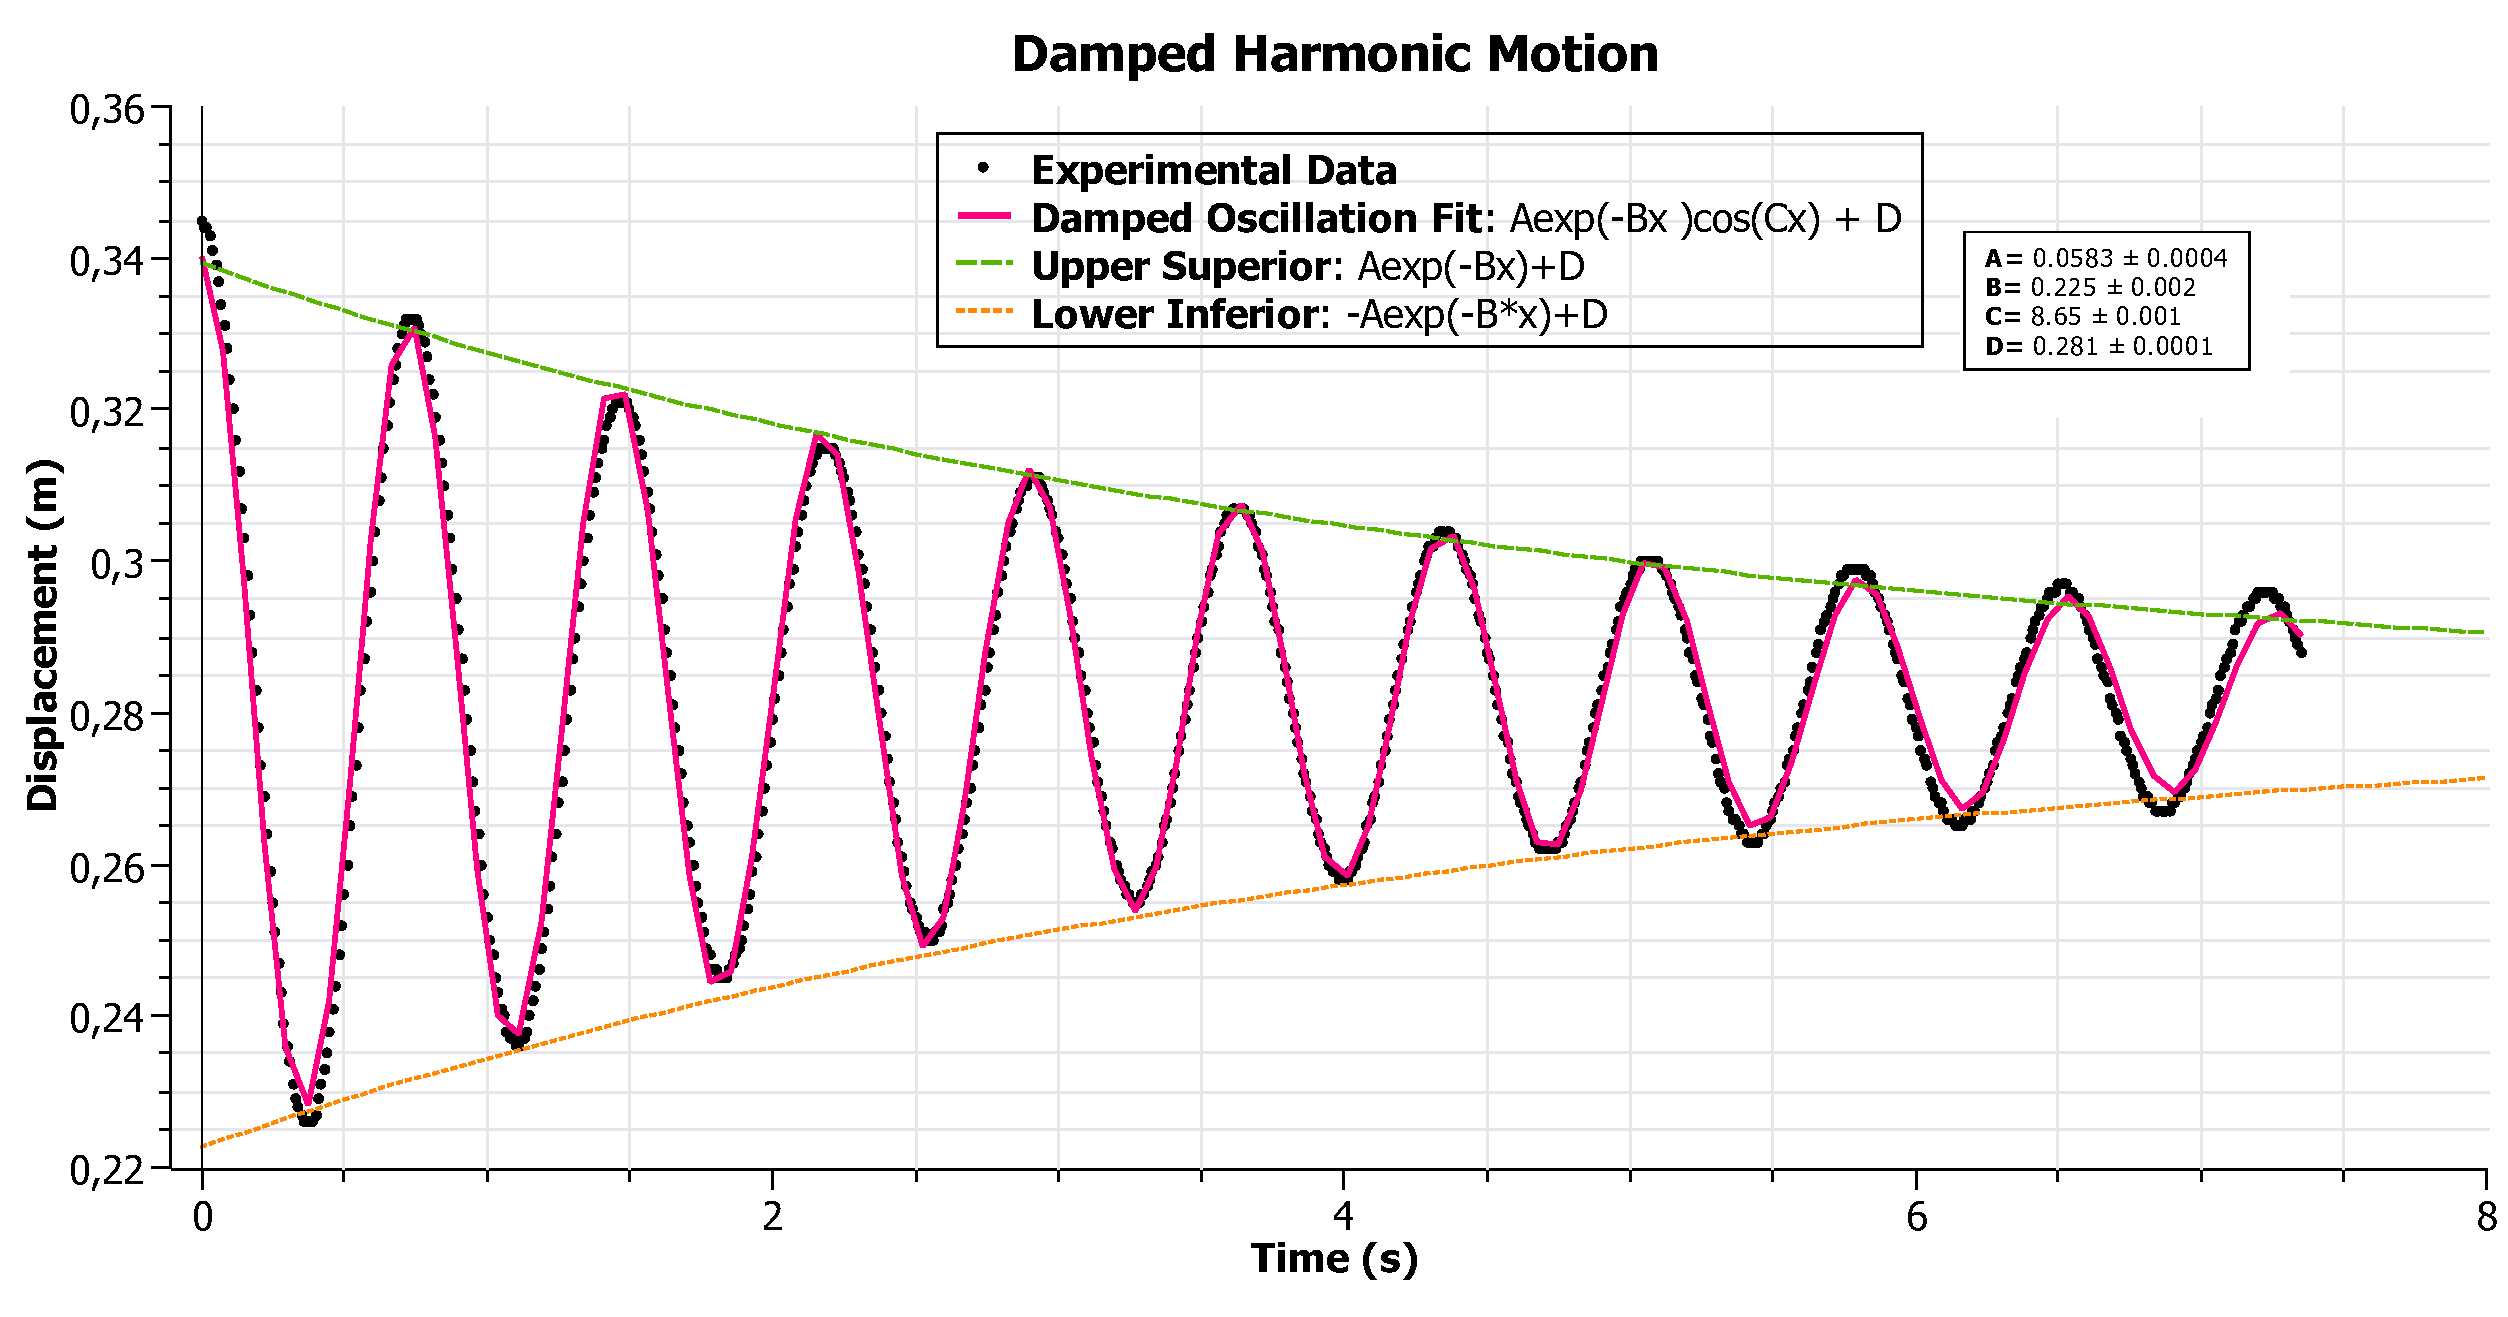
\includegraphics[width=1\textwidth]{media/graphs/damped_oscilation}
\caption{Ajuste Não Linear da Oscilação Amortecida e Envelopes. Fonte: Autor}
\label{fig:ajuste_nao_linear_amortecida}
\end{figure}


\subsubsection{Log do SciDAVis Para o Movimento Oscilatório Amortecido}

\begin{verbatim}
[Friday, 15 May 2026 18:25:19 Hora oficial do Brasil	Plot: ''Graph1'']
Non-linear fit of dataset: Table1_2, using function: a * exp(-b*x ) * cos(c*x) + d
Y standard errors: Unknown
Scaled Levenberg-Marquardt algorithm with tolerance = 1e-06
From x = 0 to x = 7.3498
a  = 0.0583143741288755 +/- 0.000416281073056886
b  = 0.225335669514056 +/- 0.00278163594869789
c  = 8.65000462658711 +/- 0.00184265354845219
d  = 0.281866484118054 +/- 0.000104600331507664
--------------------------------------------------------------------------------------
Chi^2 = 0.00589196240686965
R^2 = 0.999900004546549
---------------------------------------------------------------------------------------
Iterations = 14
Status = success
---------------------------------------------------------------------------------------
\end{verbatim}

Utilizando a totalidade de pontos discretos oscilação amortecida no SciDAVis, aplicou-se uma regressão não linear por meio por meio da ferramenta \textit{Fit Wizard}, utilizando a função de ajuste:
\begin{equation}
    y = A\exp(-Bx)\cos(Cx + D)
\end{equation}
Onde as variáveis de ajuste mapeiam os parâmetros físicos da seguinte forma: $A \equiv A_0$, $B \equiv \beta$, $C \equiv \omega$ e $D \equiv \phi_0$.
\begin{itemize}
    \item $A = \SI{0.0583 \pm 0.0004}{\meter}$
    \item $B = \SI{0.225 \pm 0.002}{\second^{-1}}$
    \item $C = \SI{8.65 \pm 0.001}{\text{rad}/\second}$
    \item $D = \SI{0.281 \pm 0.0001}{\text{rad}}$
\end{itemize}

Com os valores encontrados para $A$, $B$, e $D$, foram construidos as curvas de envelope seguindo a equação \ref{eq:envelope}.

E utilizando a tabela de pontos mínimos e máximos, foram aplicados ajustes não lineares para as funções de envelope, utilizando a função de ajuste:


\begin{table}[H]
    \centering
    \caption{Tabela de pontos mínimos e máximos para o ajuste dos envelopes. Fonte: Autor}
    \label{tab:tabela_min_max}
    \begin{tabular}{cccc}
        \toprule
        \multicolumn{2}{c}{\textbf{Mínimos}} & \multicolumn{2}{c}{\textbf{Máximos}} \\
        \cmidrule(lr){1-2} \cmidrule(lr){3-4}
        Tempo (s) & Posição (m) & Tempo (s) & Posição (m) \\
        \midrule
        0.3697 & 0,226 & 0.0000 & 0,345 \\
        1.0997 & 0,236 & 0.7300 & 0,332 \\
        1.8297 & 0,245 & 1.4599 & 0,321 \\
        2.5497 & 0,250 & 2.1699 & 0,315 \\
        3.2697 & 0,255 & 2.9099 & 0,311 \\
        3.9998 & 0,258 & 3.6199 & 0,307 \\
        4.6998 & 0,262 & 4.3399 & 0,304 \\
        5.4198 & 0,263 & 5.0499 & 0,300 \\
        6.1398 & 0,265 & 5.7699 & 0,299 \\
        6.8798 & 0,267 & 6.5299 & 0,297 \\
        --     & --    & 7.2199 & 0,296 \\
        \bottomrule
    \end{tabular}
\end{table}

Com a tabela de máximos e mínimos, foram aplicados ajustes não lineares para as funções de envelope, utilizando a função de ajuste:
\begin{equation}
    y = A\exp(-Bx) + D
\end{equation}

\begin{figure}[H]
\centering
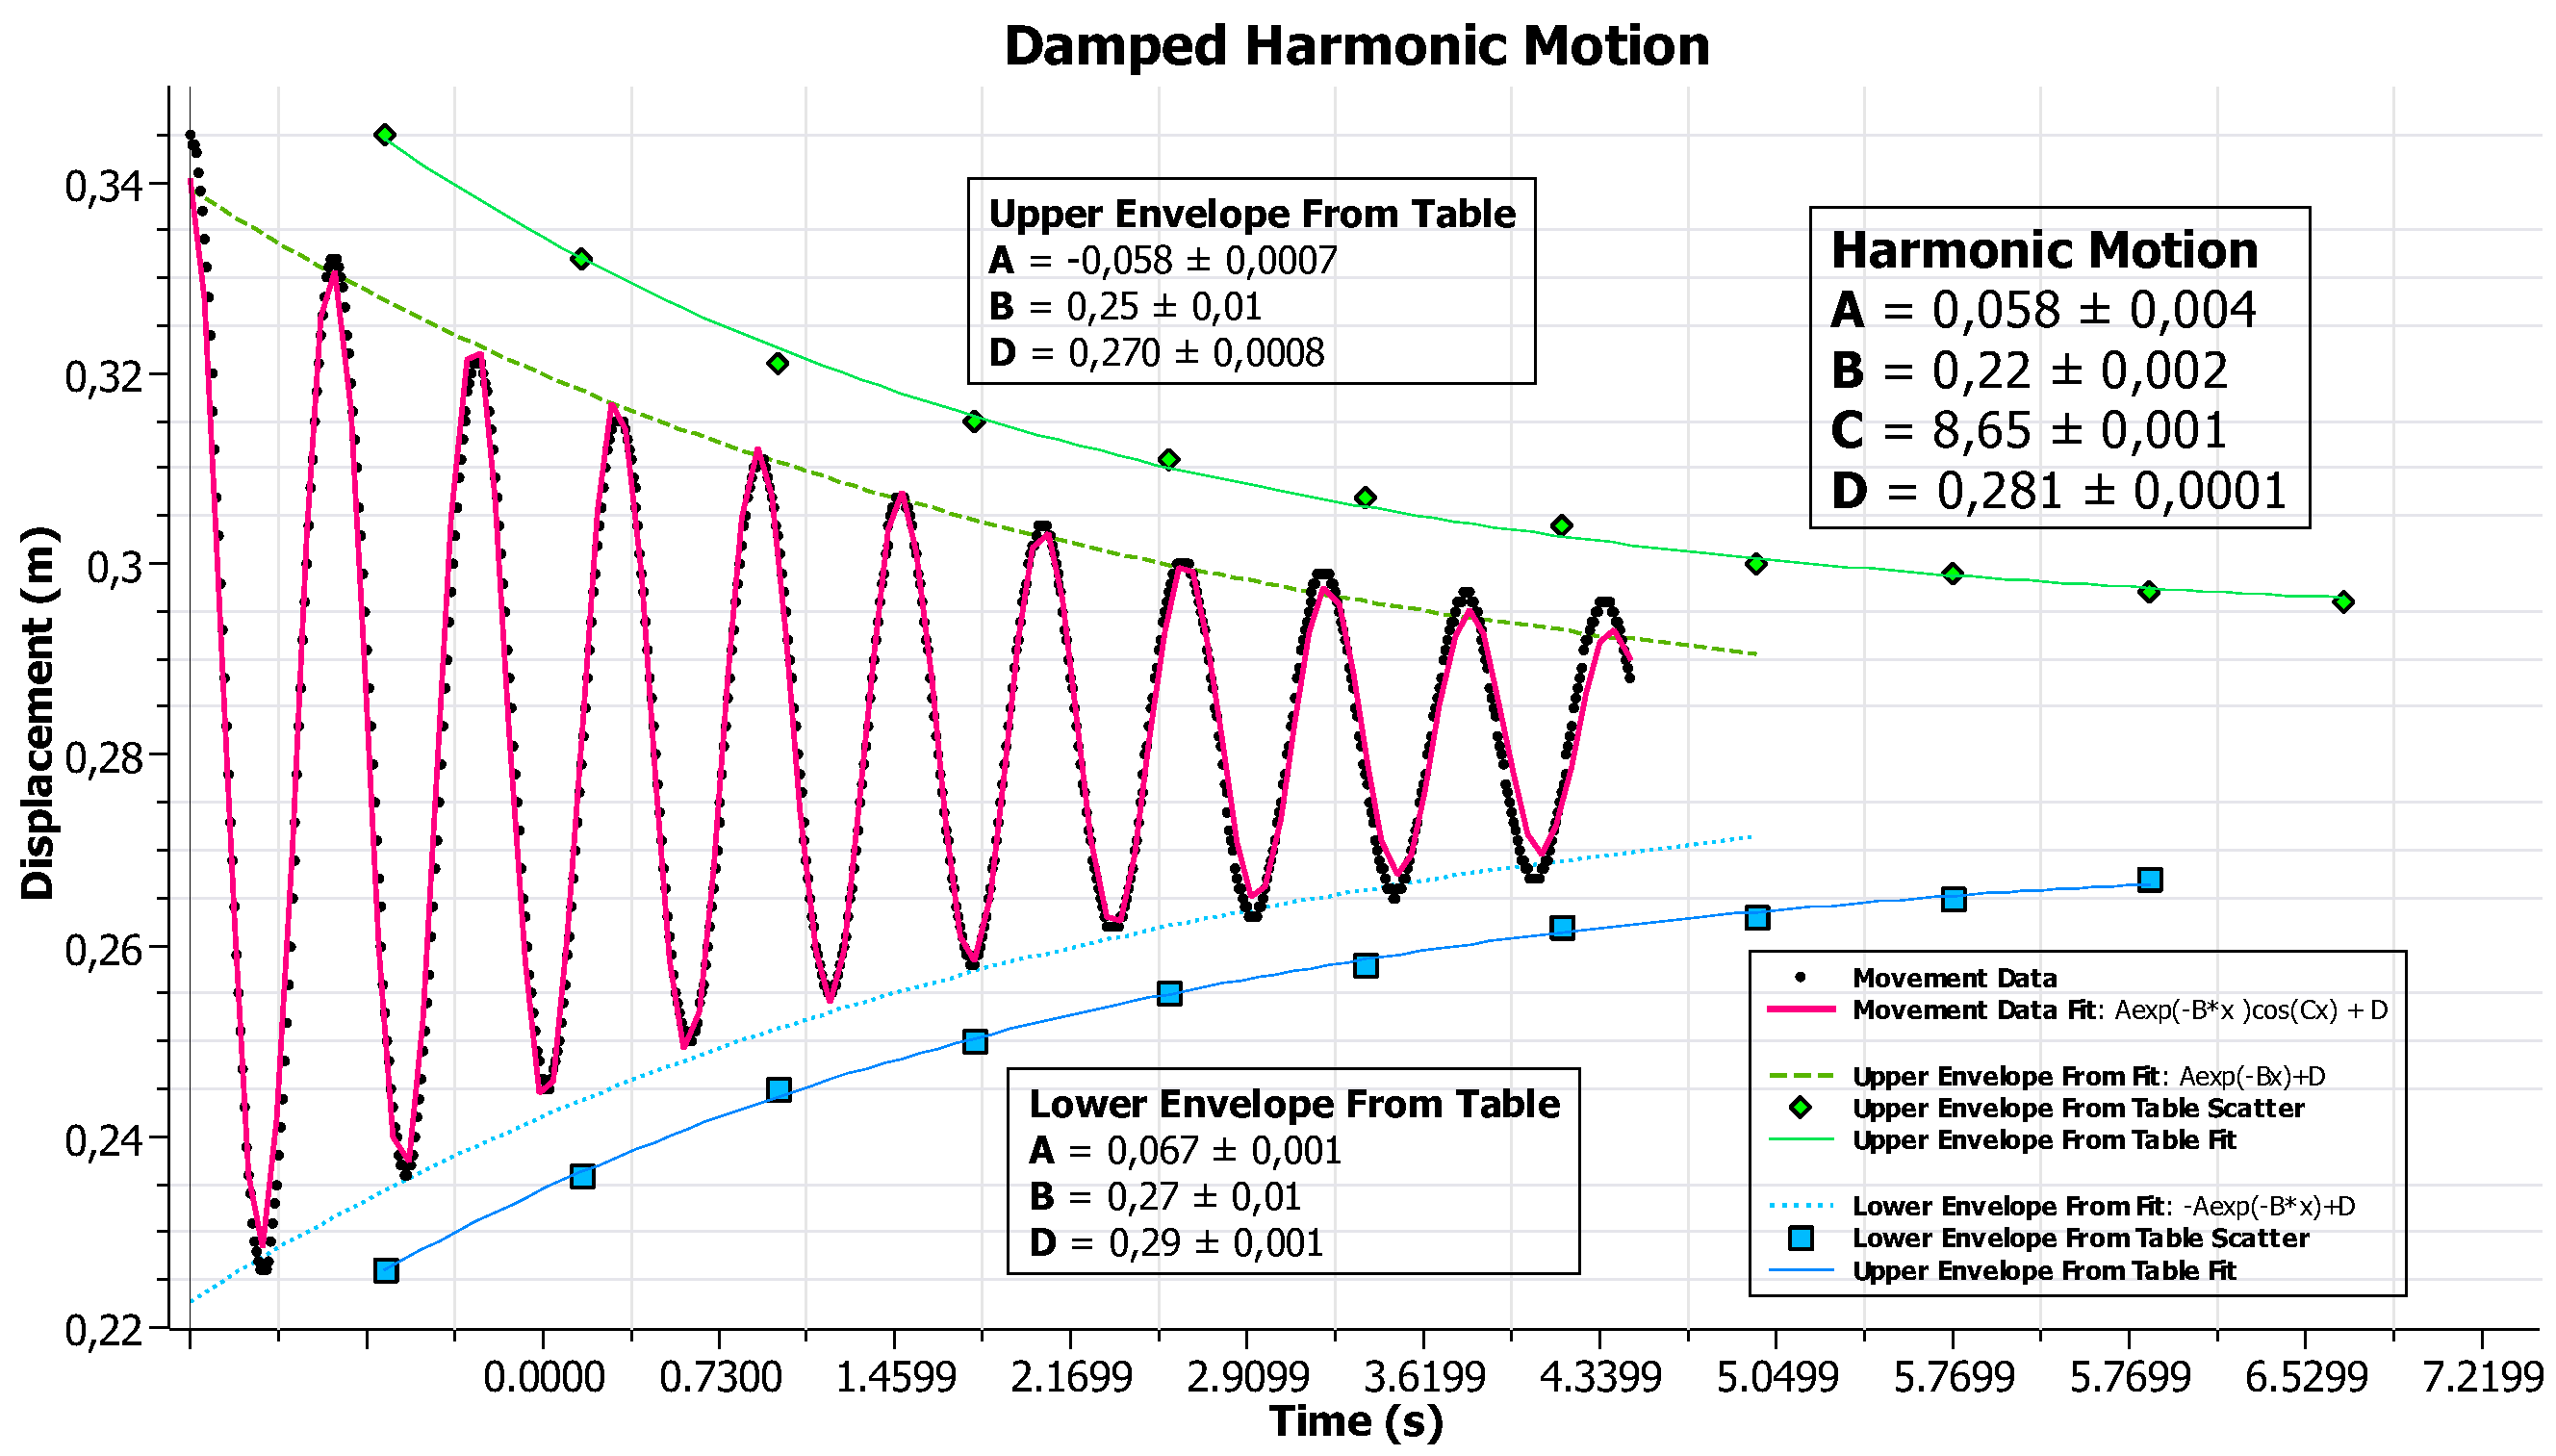
\includegraphics[width=1\textwidth]{media/graphs/damped_oscilation_with_envelopes}
\caption{Ajuste Não Linear da Oscilação Amortecida e Envelopes. Fonte: Autor}
\label{fig:ajuste_nao_linear_amortecida_envelopes}
\end{figure}

\subsubsection{Log do SciDAVis Para o Envelope}

\begin{verbatim}
[sexta-feira, 22 de maio de 2026 11:51:26 Hora oficial do Brasil	Plot: ''Graph1'']
Non-linear fit of dataset: Table1_MIN 1, using function: a * exp(-b*x ) + d
Y standard errors: Unknown
Scaled Levenberg-Marquardt algorithm with tolerance = 0,0001
From x = 1 to x = 10
a  = -0,0580402460219572 +/- 0,00079844963184216
b  = 0,259153103884351 +/- 0,0126235289855455
d  = 0,270849724140474 +/- 0,000852758377517397
--------------------------------------------------------------------------------------
Chi^2 = 2,15380538231939e-06
R^2 = 0,999996635798738
---------------------------------------------------------------------------------------
Iterations = 30
Status = success
---------------------------------------------------------------------------------------
[sexta-feira, 22 de maio de 2026 11:51:40 Hora oficial do Brasil	Plot: ''Graph1'']
Non-linear fit of dataset: Table1_MAX 1, using function: a * exp(-b*x ) + d
Y standard errors: Unknown
Scaled Levenberg-Marquardt algorithm with tolerance = 0,0001
From x = 1 to x = 11
a  = 0,0675528369909234 +/- 0,00135788065562808
b  = 0,278184329080995 +/- 0,0164536362542707
d  = 0,293295722215092 +/- 0,00103993350263416
--------------------------------------------------------------------------------------
Chi^2 = 6,89448504195265e-06
R^2 = 0,999993557320727
---------------------------------------------------------------------------------------
Iterations = 4
Status = success
---------------------------------------------------------------------------------------
\end{verbatim}

A partir do valor encontrado para $B$, é possível determinar a constante de amortecimento $\beta$ e, consequentemente, a frequência angular $\omega$ do sistema.
\begin{align*}
    B &= 2\beta \\
    \beta &= \frac{B}{2}\\ 
    \implies \gamma &= 2\beta \\
    &= 2 \times 0.1125 = 0.225 \, s^{-1}
\end{align*}

Então, a constante de amortecimento do sistema, $\gamma$ que indica a taxa de decaimento da amplitude da oscilação é igual a $0.225 \, s^{-1}$.

O valor encontrado para $C$ corresponde à frequência angular da oscilação, que é dada por:
\begin{align*}
    C &= \omega \\
    \omega &= 8.65 \, \text{rad/s}
\end{align*}

\section{Discussão}

\subsection{Período e Frequência Angular a partir dos Máximos}

A partir dos valores de tempo registrados na Tabela~\ref{tab:tabela_min_max}, foram identificados 11 máximos da oscilação, correspondendo a 10 intervalos de período. O período médio $T$ foi calculado utilizando os instantes do primeiro e do último máximo, divididos pelo número de intervalos:

\begin{equation}
    T = \frac{t_{11} - t_1}{n-1} = \frac{7{,}2199 - 0{,}0000}{10} = \SI{0,7220}{\second}
\end{equation}

O desvio padrão dos períodos individuais foi calculado a partir dos 10 intervalos, obtendo-se $\sigma_T = \SI{0,019}{\second}$, e a incerteza da média é $\delta T = \sigma_T / \sqrt{10} \approx \SI{0,006}{\second}$. Portanto:

\begin{equation}
    T = (0{,}722 \pm 0{,}006)\,\si{\second}
\end{equation}

A frequência angular $\omega'$ foi então determinada por:

\begin{equation}
    \omega' = \frac{2\pi}{T} = \frac{2\pi}{0{,}7220} \approx \SI{8{,}703}{\radian\per\second}
\end{equation}

com incerteza propagada:

\begin{equation}
    \delta\omega' = \omega' \cdot \frac{\delta T}{T} = 8{,}703 \times \frac{0{,}006}{0{,}722} \approx \SI{0{,}07}{\radian\per\second}
\end{equation}

Portanto, $\omega' = (8{,}70 \pm 0{,}07)\,\si{\radian\per\second}$.

\subsection{Comparação dos Parâmetros dos Ajustes}

O valor de $\omega'$ obtido diretamente dos dados experimentais é consistente com o parâmetro $C = (8{,}65 \pm 0{,}002)\,\si{\radian\per\second}$ encontrado pelo ajuste não linear da curva completa no SciDAVis. A diferença relativa entre os dois é inferior a $0{,}6\%$, confirmando a coerência dos resultados.

Os demais parâmetros do ajuste da curva completa — $A = \SI{0{,}0583}{\meter}$, $B = \SI{0{,}225}{\per\second}$ e $D = \SI{0{,}282}{\meter}$ — foram comparados com os parâmetros dos ajustes dos envelopes (Tabela~\ref{tab:comparacao_parametros}).

\begin{table}[H]
    \centering
    \caption{Comparação entre os parâmetros da curva completa e dos envelopes. Fonte: Autor}
    \label{tab:comparacao_parametros}
    \begin{tabular}{lccc}
        \toprule
        \textbf{Origem} & $|A|$ (m) & $B$ (s$^{-1}$) & $D$ (m) \\
        \midrule
        Curva completa  & $0{,}0583$ & $0{,}225$ & $0{,}282$ \\
        Envelope Inferior & $0{,}0580$ & $0{,}259$ & $0{,}271$ \\
        Envelope Superior & $0{,}0676$ & $0{,}278$ & $0{,}293$ \\
        \bottomrule
    \end{tabular}
\end{table}

Observa-se que as amplitudes $|A|$ são compatíveis entre si, com diferença inferior a $16\%$. As ligeiras divergências nos valores de $B$ e $D$ entre os envelopes e a curva completa são esperadas, pois os ajustes parciais utilizam apenas 10 ou 11 pontos, sendo mais sensíveis às flutuações, enquanto o ajuste global emprega todos os pontos e apresenta $R^2 = 0{,}9999$.

\subsection{Constante de Amortecimento $b$}

Utilizando o parâmetro $B = \beta = \SI{0{,}1125}{\per\second}$ e a massa $m = \SI{0{,}11930}{\kilo\gram}$, a constante de amortecimento viscoso $b$ foi determinada pela relação $B = b/(2m)$:

\begin{equation}
    b = 2mB = 2 \times 0{,}11930 \times 0{,}1125 \approx \SI{0{,}02684}{\kilo\gram\per\second}
\end{equation}

\subsection{Comparação entre $\omega_0$ e $\omega'$}

A frequência natural de oscilação $\omega_0$ pode ser obtida a partir da relação~(4) do roteiro:

\begin{equation}
    \omega_0 = \sqrt{(\omega')^2 + \left(\frac{b}{2m}\right)^2} = \sqrt{8{,}65^2 + 0{,}1125^2} = \sqrt{74{,}8225 + 0{,}01266} \approx \SI{8{,}651}{\radian\per\second}
\end{equation}

A diferença relativa entre $\omega_0$ e $\omega'$ é:

\begin{equation}
    \frac{\omega_0 - \omega'}{\omega_0} = \frac{8{,}651 - 8{,}650}{8{,}651} \approx 0{,}01\%
\end{equation}

Esse resultado confirma que, para o sistema estudado, o amortecimento é suficientemente fraco ($\beta \ll \omega'$) para que a aproximação $\omega_0 \approx \omega'$ seja plenamente válida. Em termos físicos, isso significa que a resistência do fluido (ar) afeta a amplitude das oscilações, mas não altera perceptivelmente a frequência do sistema. Esse regime caracteriza o chamado \textbf{subamortecimento fraco}, onde a energia dissipada por ciclo é pequena em relação à energia total armazenada no sistema.


\bibliographystyle{plainnat}
\bibliography{refs}

\end{document}